\documentclass[10pt,a4paper]{article}
\usepackage[latin1]{inputenc}
\usepackage{amsmath}
\usepackage{amsfonts}
\usepackage{amssymb}
\usepackage{float}
\usepackage{listings}
\usepackage{graphicx}

\begin{document}

\lstset{language=Mathematica,breaklines=true}

\author{Jeroen Hofman\\
		10194754\\
		}
\title{Computer exercises week 38, 2011\\
		}
\date{}
\maketitle

\subsection*{Exercise 3.5}

Code:
\begin{lstlisting}
x = {1.02, 0.95, 0.87, 0.77, 0.67, 0.56, 0.44, 0.30, 0.16, 0.01};
y = {0.39, 0.32, 0.27, 0.22, 0.18, 0.15, 0.13, 0.12, 0.13, 0.15};
list = Transpose[{x, y}];
A = Table[1, {i, 10}, {j, 5}]; (*Initialize matrix*)
f = {y^2, x y, x, y, 1 - x + x};
For[i = 1, i < 11, i++, For[j = 1, j < 6, j++, A[[i, j]] = f[[j, i]]]]; (*Fill matrix*)
r = x^2;

coef = LeastSquares[A, r]; (*Use least squares routine*)

x2 = x + RandomReal[{-0.005, 0.005}, Length[x]];
y2 = y + RandomReal[{-0.005, 0.005}, Length[y]]; (*Adjust data*)
list2 = Transpose[{x2, y2}];
f = {y2^2, x2 y2, x2, y2, 1 - x2 + x2};
For[i = 1, i < 11, i++, For[j = 1, j < 6, j++, B[[i, j]] = f[[j, i]]]];

q2 = x2^2;

coef2 = LeastSquares[B, q2];

\end{lstlisting}

\noindent In this exercise we are given a set of data points (x,y) and we compute the coefficients of the elliptic trajectory, given by ay$^2$ + bxy + cx + dy + e = x$^2$. We use Mathematica to construct a matrix out of the problem, where each i-th row of the matrix is of the form \{y$_{i}^{2}$,x$_{i}$y$_{i}$,x$_{i}$,y$_{i}$,1\} where x$_{i}$ and y$_{i}$ are the i-th pair of data points. Then the problem is solved by a Mathematica routine which implements least squares. The resulting coefficients are a = -2.6356, b = 0.1436, c = 0.5514, d = 3.2229, e = -0.4329. Then we perturb the data slightly by adding a random number between [0.005,-0.005] to every datapoint. We use the same procedure to obtain the coefficients, which are a = -3.6022, b = 0.8164, c = 0.4479, d = 3.0663, e = -0.3855. So the coefficients are affected by this small change in the input of the data. The figure below shows the given data points together with the first fit, which is the small ellipse. The big ellipse is the result of the second fit, with the slightly perturbed data (the perturbed data points are not visible, because they overlap with the original ones). So we can conclude that a small perturbation gives a large difference in the trajectory of the object. The reason is that the data points only describe a small portion of the total ellipse, which causes the small local change in curvature to be magnified throughout the rest of the ellipse. If the data points would have been distributed evenly on the trajectory, then small perturbations wouldn't have altered the object's trajectory that much.

\begin{figure}[H]
\centering
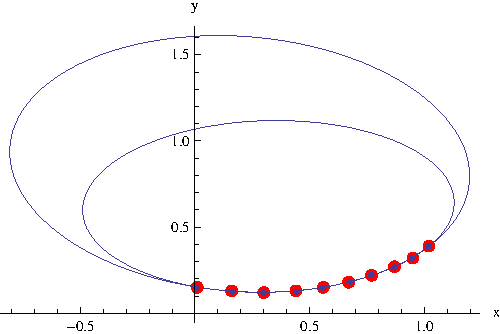
\includegraphics[scale=1.5]{3_5.pdf}
\end{figure}

\subsection*{Exercise 3.10}
\lstset{language=Python}
Code:
\begin{lstlisting}
#Generate random matrix A
m = random.randint(3,10)
n = random.randint(m,10)
A = np.random.randn(n,m)

#QR decomposition of A
(Q,R) = np.linalg.qr(A)
R_t = np.transpose(R)

#Compute inverse of R
R_inv = np.matrix(np.zeros([m,m]))
for i in range(0,m):
    R_inv[i,i] = 1/R[i,i]
for i in range(0,m):
    for j in range(i+1,m):
        R_inv[i,j] = 0
        for k in range(i,j):
            R_inv[i,j] -= R_inv[i,k]*R[k,j]
        R_inv[i,j] /= R[j,j]
R_t_inv = np.transpose(R_inv)

#Compute covariance matrix and compare with (A^T A)^-1
print np.dot(R_inv,R_t_inv)
print inv(np.dot(np.transpose(A),A))
\end{lstlisting}

\noindent In this exercise the goal is to calculate the covariance matrix given by $\sigma^{2}(A^{T}A)^{-1}$, where we choose $\sigma = 1$. If we do a QR factorization of A we see that the covariance matrix can be written as $(A^{T} A)^{-1} = ((QR)^{T} QR)^{-1} = (R^{T}Q^{T}QR)^{-1} = (R^{T}R)^{-1}$, using the fact that Q is orthogonal. Note furthermore that $(R^{T}R)^{-1} = R^{-1} (R^{T})^{-1} = R^{-1} (R^{-1})^{T}$, so given R from the QR factorization of A, the only thing we need to do is to invert R. The code above generates a random nxm matrix A, uses a library routine for QR factorization and then computes the inverse of R. In the end it prints both $(R^{T}R)^{-1}$ and $(A^{T}A)^{-1}$ to check if they indeed do the same results. I've checked it for 10 different matrices of different sizes (up to 10x10) and in all cases $(R^{T}R)^{-1} = (A^{T}A)^{-1}$, so the method of computing the covariance matrix given only R is indeed correct. An example is given below.\\
\\
\begin{center}
$A = 
\begin{pmatrix}
-0.35108121&-0.02332135&1.01264486\\
-1.04893079&0.04761579&-0.78089814\\
1.83696179&1.05729834&0.718104\\
\end{pmatrix}
$
\\
$R = 
\begin{pmatrix}
2.14428133&0.88629167&0.83138211\\
0.&-0.5789456&0.0663209\\
0.&0.&1.20637068\\
\end{pmatrix}
$
\\
$(A^{T}A)^{-1} = (R^{T}R)^{-1} = 
\begin{pmatrix}
0.85725163&-1.26740584&-0.29894884\\
-1.26740584&2.99250631&0.07871384\\
-0.29894884&0.07871384&0.68712928\\
\end{pmatrix}
$
\end{center}

\end{document}